\documentclass[12pt]{article}
%\usepackage[scaled]{helvet}
\usepackage{amsmath}
\usepackage[utf8]{inputenc}
\usepackage{graphicx}
\usepackage{url}
\usepackage[font={small,it}]{caption}
%\renewcommand\familydefault{\sfdefault}
%\renewcommand{\baselinestretch}{1.1}
\usepackage[letterpaper, margin=1in]{geometry}
\usepackage{listings}
\lstset{basicstyle=\tiny,language=Python}

\newcommand\figref[1]{Fig.~\ref{fig:#1}}

\title{Udacity Machine Learning Nanodegree\\ CAPSTONE: Photo OCR Prototype}
\author{Wolfgang Steiner \\ \small{wolfgang.steiner@gmail.com}}
\date{January 2017}

\begin{document}
\maketitle
\section{Introduction}
In this capstone project I present the prototype of a photo OCR (optical character recognition)
pipeline based on a sliding window algorithm that is able to automatically detect and parse
text in images. Systems such as this are used in a wide variety of applications
such as the automatic parsing of house numbers from street view photos \cite{Goodfellow2013},
automatic translation of text \cite{} or scanning of documents using a mobile device \cite{}.

The task of photo OCR can be divided into three distinct stages which are shown in \figref{pipeline}.
The first stage of this pipeline is \emph{text detection} which aims to determine bounding boxes for each
distinct set of characters in the image. The second stage is \emph{character segmentation}, in which
each bounding box is scanned for character boundaries with the aim of finding distinct characters
that can finally be classified in the third stage by the \emph{character classification}.

{\bf[TODO]}
Each stage of the pipeline consists of a convolutional neural network

In order to reduce the complexity and training time of the project, the pipeline is confined to
only process and parse digits but every stage could be extended and retrained to also handle letters
and other characters.

Similar to the work in \cite{Jaderberg2016} synthetic images have been generated to train the classifiers.


\begin{figure}[ht]
    \centering
    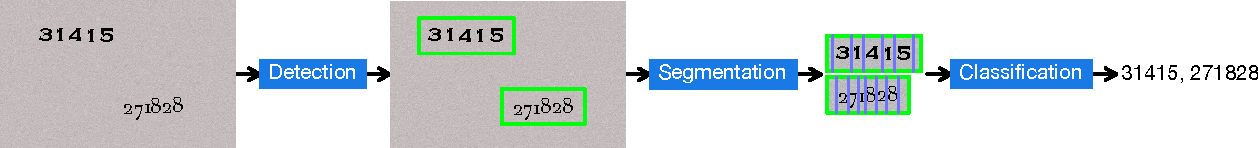
\includegraphics[scale=0.8]{fig/Pipeline}
    \caption{Photo OCR pipeline.}
    \label{fig:pipeline}
\end{figure}

\section{Metrics and Benchmark}
In order to assess the performance of the complete OCR pipeline, a set of test images $x_i$ containing
a randomly generated string of digits of varying length is processed and the extracted string $a(x_i)$ is
compared to the real label $y(x_i)$ using the following metric:
\begin{equation}
  \operatorname{accuracy}(\begin{bmatrix}x_{1}\\x_{2}\\\vdots\\x_{n}\end{bmatrix},\begin{bmatrix}y(x_{1})\\y(x_{2})\\\vdots\\y(x_{n})\end{bmatrix}) = 1 - \frac{\sum\limits_{i=0}^n{\operatorname{min}\left(\operatorname{lev}(y(x_i), a(x_i)), |y(x_i)|\right)}}{\sum\limits_{i=0}^n{|y(x_i)|}}
\end{equation}
Here, $a(x_i)$ is the label (string of digits) predicted by the system and $|y(x_i)|$ is the length of
the i-th true label. $\operatorname{lev}(y(x_i), a(x_i))$ denotes the Levenshtein distance \cite{Levensht20:online} between
the true label and the predicted label. The Levenshtein distance counts the number of edit operations
that are required to make two strings exactly equal by either deleting, inserting or
changing single characters. When calculating the accuracy, the Levenshtein distance is limited to
the length of the true label (by use of the $\operatorname{min}$ function). This prevents the accuracy
of a single example to become negative.

Human level performance on the task of text transcription is often estimated to be greater
than 98\% \cite{Goodfellow2013}. So an obvious benchmark for a OCR system would be to
attain comparable or even better performance than a human is capable of. When extracting text the
performance of the system can be augmented by use of a dictionary to correct badly classified
characters. When dealing with number strings only, this augmentation is not possible and
the accuracy of the OCR system

A second performance benchmark is speed. One application for an OCR system would be text extraction
of documents scanned by use of the camera of a smartphone. The images would then be send to
a server for processing or even better would be precessed directly on the mobile device.
In both cases scanning a photo for text should not take more than a few second. For use in
an augmented reality app, the speed needs to be even faster in order to allow for an acceptable
frame rate. In this case, processing on the mobile device should be faster than about
250ms.


\section{Training Data}
In this project I predominantly used synthetic images. In order to have a large variety of fonts,
I used the google fonts repository as a source \cite{googlefo53:online}. After excluding some
symbol and non-latin fonts, a collection of 1747 fonts was available for synthesizing images.
The procedure for synthesizing training images is as follows:

\begin{figure}[ht!]
  \centering
  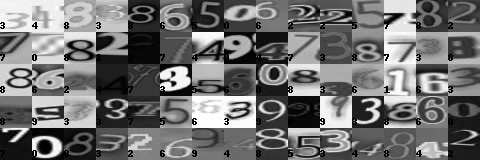
\includegraphics[width=1.0\linewidth]{fig/training_example_images/classifier}
  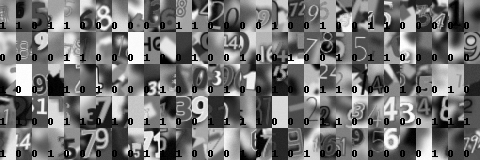
\includegraphics[width=1.0\linewidth]{fig/training_example_images/segmentation}
  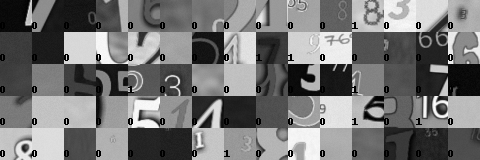
\includegraphics[width=1.0\linewidth]{fig/training_example_images/detection}
  \caption
  {
    Examples of synthesized images used to train the character classifier (top),
    character segmentation classifier (center) and character detection classifier (bottom).
  }
  \label{fig:training_images}
\end{figure}

\begin{itemize}
  \itemsep0em
  \item A text and a background color is chosen randomly.
  \item A background image is synthesized by upscaling noise by a random factor and applying gaussian blurring.
  \item One of the 1747 fonts is chosen randomly.
  \item One of the characters is chosen randomly.
  \item Adjacent characters are added in some images to the left or right.
  \item An outline is randomly added to the characters.
  \item A shadow of random width and direction is added to the characters.
  \item The image is rotated by a random amount.
  \item Gaussian blur is applied with random radius.
  \item White noise of random amount is added to the image.
\end{itemize}



Some examples of images used to train the three required CNN classifiers are shown in \figref{training_images}.
%
In all cases, training and prediction is done with grayscale images with a fixed height of 32~pixels.
%
Training images are not pre-generated before training but are generated online during training.
%
For this I implemented python generators for the three types of training images that synthesize
batches of images in separate worker threads.
%


Training images for the character classifier (\figref{training_images}, top) have characters centered in the images (32x32~pixels) as will be encountered
by the classifier after segmentation.
%
Characters are also resized to the width of the image as the windows between character boundaries are rescaled to the
input width of 32~pixels.
%
The labels are simply the corresponding character and are one-hot encoded for training and prediction.


Training images for the segmentation classifier (\figref{training_images}, center) are only 16~pixels wide in order to improve the spacial resolution of the segmentation procedure (see below).
%
Here, label "1" is assigned if a character starts to the right of the center (for the beginning of a character sequence),
a character starts to the left of the center (for the end of a character sequence), or if the spacing
between characters is in the center of the image (for segmenting between characters of a sequence).
%
Label "0" is assigned, if no character is present in the image or if a character is in the center of the image.


Finally, the training images for the character detection classifier (\figref{training_images}, bottom) are
designed to find bounding boxes for character sequences that fit as tightly as possible in order to improve
the accuracy of character segmentation and classification.
%
Because of this, images that only have small
text areas and images without characters are labeled "0".
%
Only images that have a high percentage of their area filled by character geometry are labeled "1".

\section{Algorithms and Techniques}
\subsection{Text Detection}
The first step in the OCR pipeline is text detection.
%
Here, a two dimensional sliding window algorithm with a window size of 32x32~pixels is used to detect characters in the image and to fit bounding boxes
around each character sequence encountered.
%
In order to detect text of different sizes, the process of sliding windows is repeated at different
scales.
%
The choice of minimum and maximum scale factors are application specific and directly determine the
biggest/smallest size of text that can be recognized and processed by the following stages of the
pipeline.
%
When scaling the image for one iteration of the sliding window procedure, it is also rescaled
so that its width and height are multiples of 32~pixels, which is the input size of the character detection
classifier.

The image data of each window is then concatenated into an input tensor for the character detection
classifier which has a sigmoid activation function at its output.
%
If the predicted value for a window exceeds a certain threshold (0.75) it is added to a rectangle list that computes
the union of overlapping rectangles.
%
At the end of the procedure, each union of positively classified rectangles is likely to be a bounding
box containing a character sequence which is subsequently segmented into single characters for classification.

In order to improve performance a very simple CNN classifier has been trained for text detection (\figref{detection_cnn}).
It consists of two convolutional layers with rectified linear units (ReLU) as activations. After
each convolutional layer, a max pooling layer reduces the size of the tensor by a factor of two.
The flattened output of the last pooling layer is then fed into two fully connected hidden layers
with 128 output neurons each. Again, ReLU is used as activation. The output layer has just one
output neuron and has a sigmoid activation layer following it. The output value of the network
will approach zero if the respective input window does not contain text and one if it does.

\begin{figure}[ht]
  \centering
  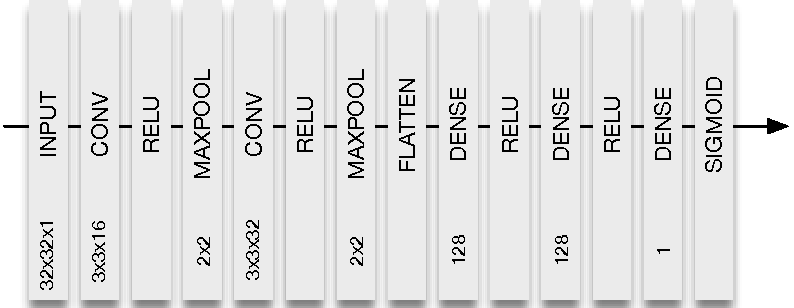
\includegraphics[scale=0.75]{fig/Detection_CNN}
  \caption
  {
    Convolutional neural network architecture of the character detection classifier.
  }
  \label{fig:detection_cnn}
\end{figure}

\subsection{Character Segmentation}
Character segmentation is based on a one-dimensional sliding window algorithm. In order to
increase the spacial accuracy of the algorithm and to reduce the number of false positives
for very narrow characters, the width to the sliding window is halved to 16~pixels in comparison
to the text detection window, while the height is equal at 32~pixels.

In a first step, the text bounding box to be processed is proportionally rescaled to a height of 32~pixels.
Then, in order to reliably detect the first and final character borders, even if the first/last
characters are close to the left/right borders of the bounding box, the image is extended by
half of the segmentation window's width (8~pixel) on the left and right side by repeating the first/last
pixel column.

The segmentation window is then moved with a one pixel increment from the left towards the right
edge of the rescaled bounding box. At every iteration, the pixel data of the window is concatenated
into an input tensor for the character segmentation CNN classifier. After evaluating the
tensor, a vector is obtained which has the score of range $[0,1]$ of the classifier's sigmoid output activation
for each pixel of the sliding window iteration.

In order to reduce the number of false positives, the segmentation score is then filtered by
a simple first order IIR filter \cite{Infinite55:online} with a filter constant of $0.5$. On this
filtered score, a simple peak detection algorithm finally locates the character boundaries at
the center of the peaks of the classifier activations (cf.~\figref{segmentation}).

\begin{figure}[ht]
    \centering
    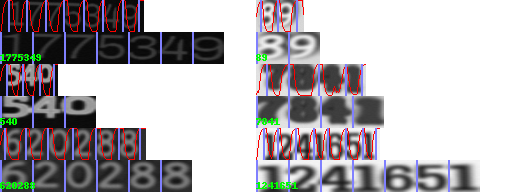
\includegraphics[width=1.1\linewidth]{fig/segmentation}
    \caption{
      Examples of the character segmentation. The top row of each example shows the input
      image. The score of the segmentation classifier is visualized in red, with each dot representing
      the output for one sliding window iteration. The resulting character border is shown in green.
      The bottom row shows the character images that have been extracted and rescaled based on the
      segmentation. These images are then fed into the character classifier. }
    \label{fig:segmentation}
\end{figure}

The architecture of the CNN classifier used for segmentation is shown in \figref{segmentation_cnn}.
In comparison to the text detection classifier, the network had to be extended in order
to achieve an acceptable segmentation accuracy. It consists of six convolutional layers
with ReLU activation with max pooling layers after each second layer. The two fully connected
hidden layers also where doubled in size. The output layer, again, has one output neuron
with sigmoid activation. The increased complexity of this classifier does not have as
great an impact on performance because it is only evaluated on the final rescaled text bounding boxes
and not on the whole input image.

\begin{figure}[ht]
  \centering
  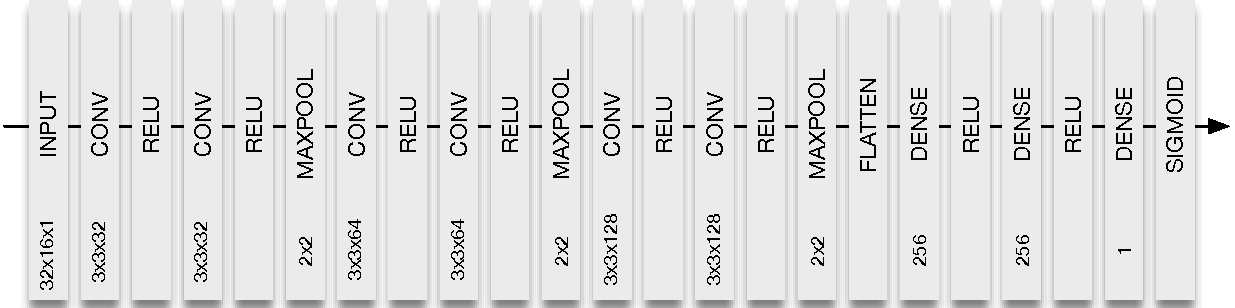
\includegraphics[scale=0.75]{fig/Segmentation_CNN}
  \caption
  {
    Convolutional neural network architecture of the character segmentation classifier.
  }
  \label{fig:segmentation_cnn}
\end{figure}



\subsection{Character Classification}
In comparison, the final stage of the OCR pipeline is rather straight-forward. At this point
in time, a list of character boundaries is available for each text bounding box. From this list,
the pixel data for each character candidate is rescaled to an image of size 32x32~pixels.

The architecture of the character classifier is shown in \figref{classifier_cnn} and is
quite similar to the segmentation classifier. The structure of the convolutional layers is
identical (apart from the different shape of the input tensor), while the size of hidden
fully connected layers has been increased substantially in order to allow for the
classification of the ten distinct digits. Accordingly, the output layer has an output size
of ten and has a softmax activation function. The output of this network is a vector
with ten entries which can be interpreted as the probabilities for the ten different classes.

\begin{figure}[ht]
  \centering
  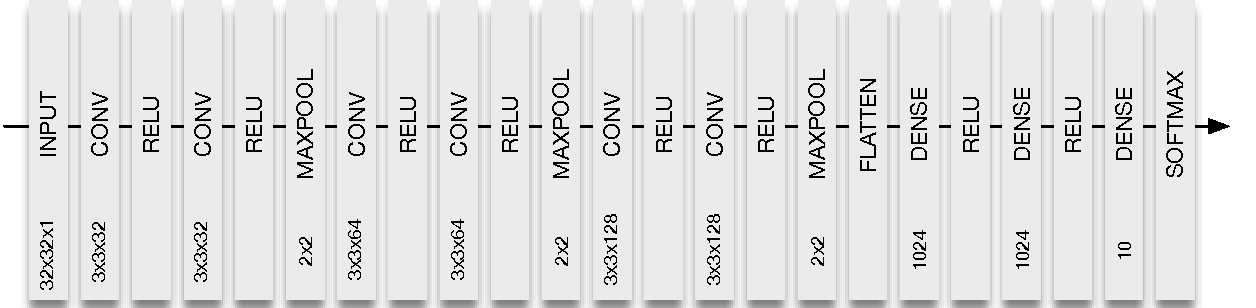
\includegraphics[scale=0.75]{fig/Classifier_CNN}
  \caption
  {
    Convolutional neural network architecture of the character classifier.
  }
  \label{fig:classifier_cnn}
\end{figure}


\section{Methodology}
In order to implement the OCR system, a bottom-up approach was used. First, the character generator
was implemented in order to synthesize training images (\figref{training_images}, top)
for the character classifier (\figref{classifier_cnn}). In order to facilitate easy and rapid
experimentation, a simple front-end was implemented that allows
for concise and expressive definitions of CNN architectures. Training data is synthesized online
during training on multiple CPU threads, using a keras generator. The classifier was trained
on a GPU (GTX 1080) using the Adam optimizer \cite{Kingma2014} and a batch size of 128.
Preprocessing simply involved normalizing the pixel values to a range of $[0, 1]$ and one-hot encoding
the labels. The epoch size is set to a rather high value of $2^{17}$ and the accuracy and categorical
cross-entropy loss on a validation set of 2048 pre-generated images is calculated. The learning rate is empirically
set to the highest value that still results in fast initial training progress and is then
successively reduced whenever the validation loss does not improve for more than four epochs.

%%\lstinputlisting[float,caption={Implementation of the character classifier CNN.},label={listing:classifier_cnn}]{../train-classifier.py}

\section{Results}
\begin{figure}[ht!]
  \begin{itemize}
    \item Accuracy of the character classifier on generated test data: 97.49\%.
    \item Accuracy of the character classifier on the svhn test data: 84.41\%.
    \item Accuracy of the segmentation classifier on generated test data: 94.70\%.
    \item Accuracy of the detection classifier on generated test data: 95.61\%.

  \end{itemize}

    \centering
    \makebox[\textwidth][c]
    {
        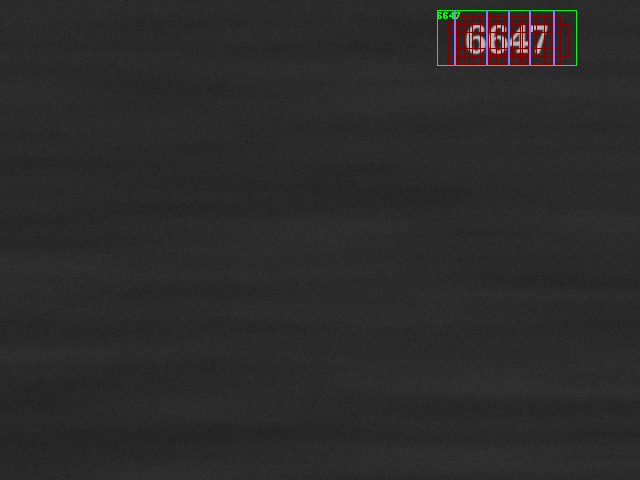
\includegraphics[width=0.35\linewidth]{fig/good_examples_pipeline/18efed02-10b7-47ce-af1e-e74a96365ea2}
        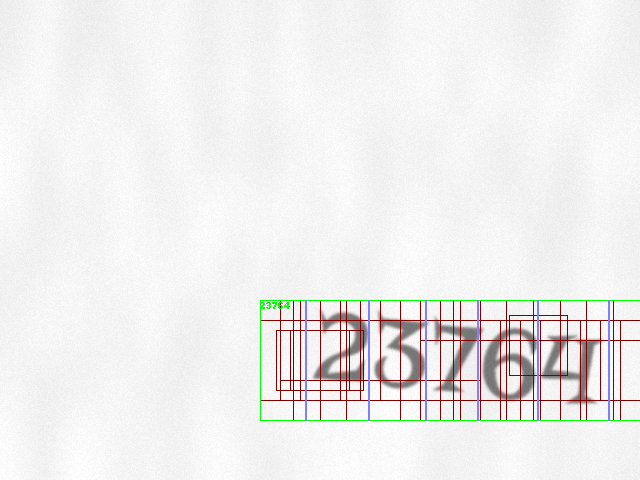
\includegraphics[width=0.35\linewidth]{fig/good_examples_pipeline/5c90c282-78f7-4432-acb0-38f245162ea9}
        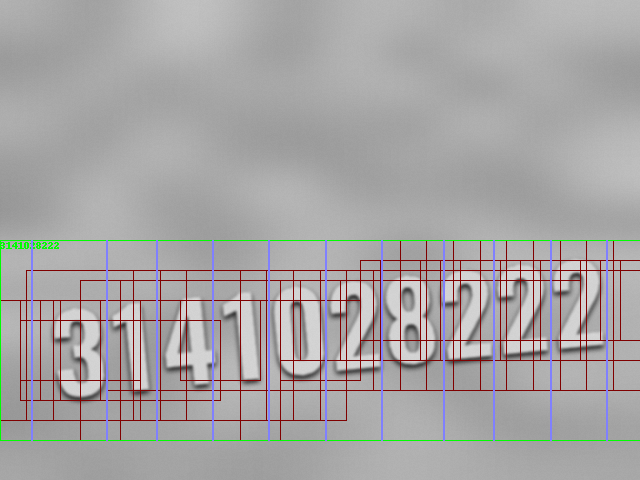
\includegraphics[width=0.35\linewidth]{fig/good_examples_pipeline/748022aa-dc7c-42d6-951b-a57db43b46b0}
    }
    \makebox[\textwidth][c]
    {
        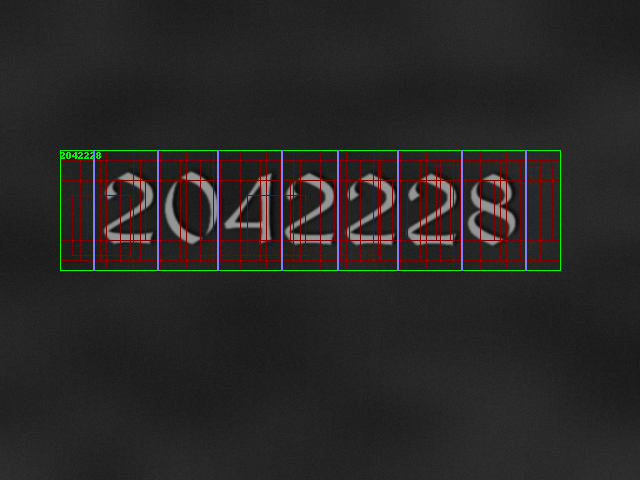
\includegraphics[width=0.35\linewidth]{fig/good_examples_pipeline/7c3ca18f-4366-40b6-8fc3-40ca42834fb9}
        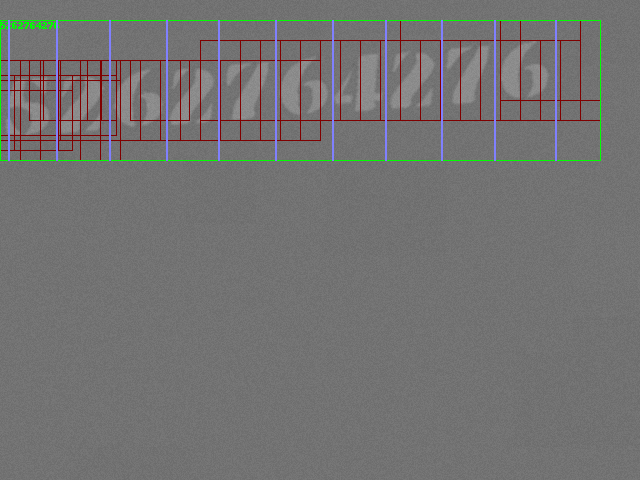
\includegraphics[width=0.35\linewidth]{fig/good_examples_pipeline/91596cec-4621-4e28-bc14-04e4815b52f9}
        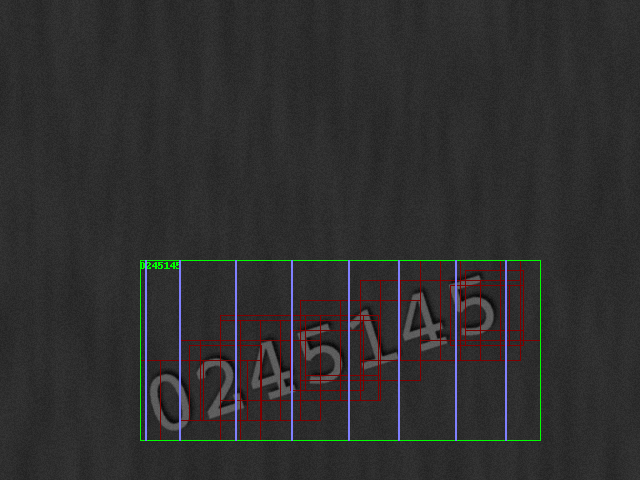
\includegraphics[width=0.35\linewidth]{fig/good_examples_pipeline/c572f505-791b-45be-bf60-9761fd9eb1b6}
    }
    \caption{Examples of correctly transcribed digit strings. Red rectangles are positive classifications of the
    character detection classifier. The green rectangle corresponds to the bounding box calculated as the union
    of the red rectangles. Boundaries between characters inferred by the segmentation algorithm are drawn in light blue.}
    \label{fig:good_examples_pipeline}
\end{figure}

\begin{figure}[ht!]
    \centering
    \makebox[\textwidth][c]
    {
        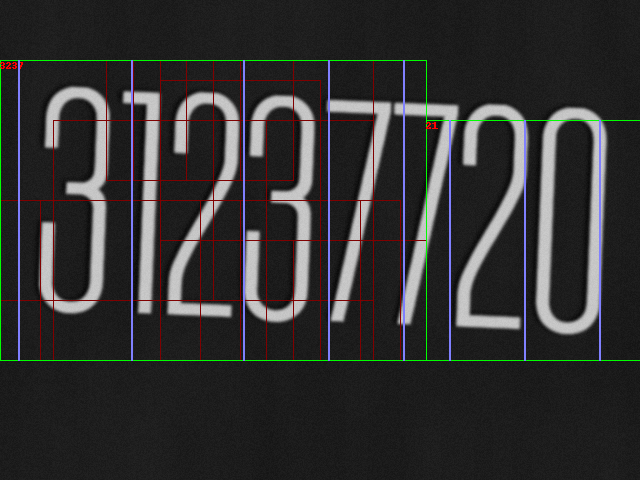
\includegraphics[width=0.35\linewidth]{fig/bad_examples_pipeline/81bde1bf-e51e-4a21-8dff-2928d5d48130}
        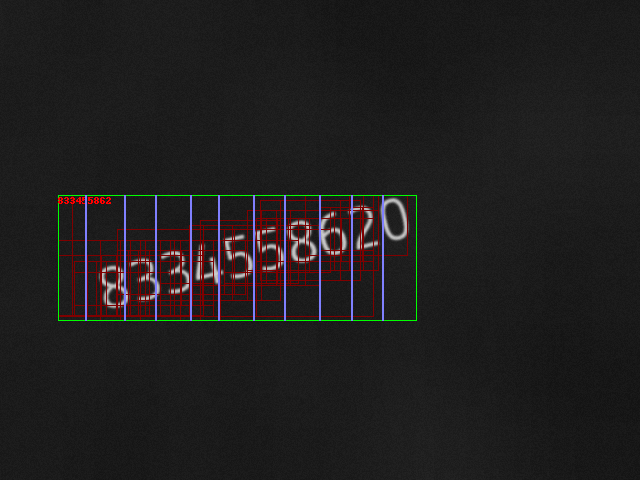
\includegraphics[width=0.35\linewidth]{fig/bad_examples_pipeline/9a566395-02bf-4676-8134-83296ded2838}
        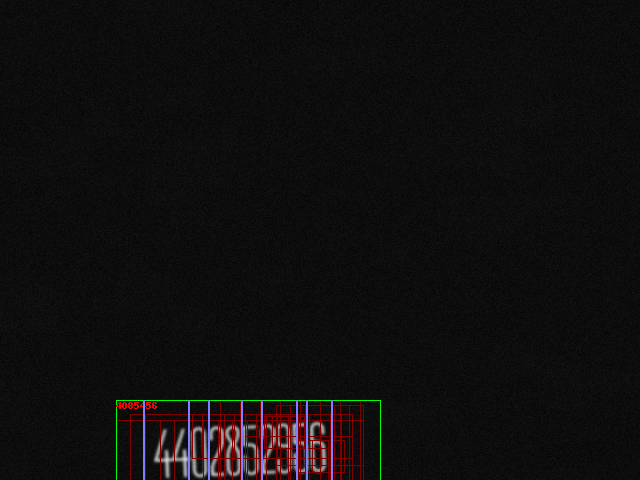
\includegraphics[width=0.35\linewidth]{fig/bad_examples_pipeline/ab748dac-6dea-41e4-9780-db48e996fd6b}
    }
    \makebox[\textwidth][c]
    {
        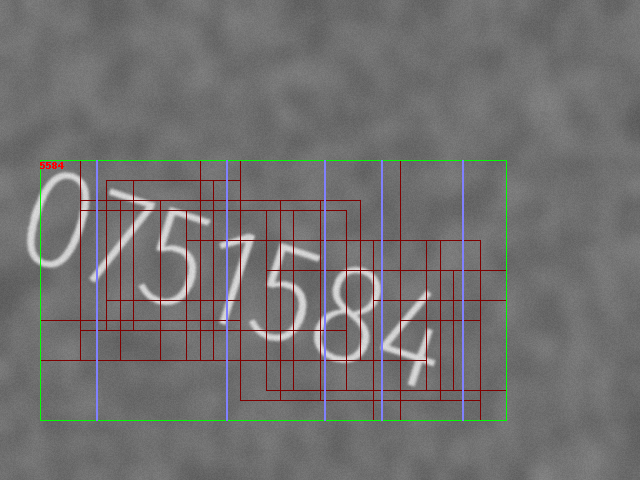
\includegraphics[width=0.35\linewidth]{fig/bad_examples_pipeline/a29de7ae-0adc-4527-b349-a317c29a6d16}
        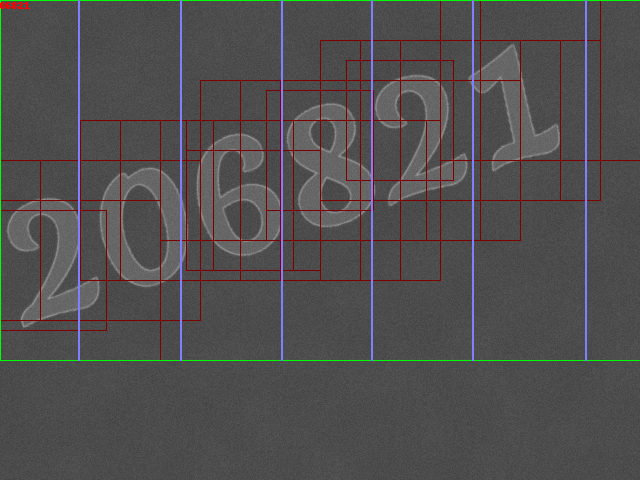
\includegraphics[width=0.35\linewidth]{fig/bad_examples_pipeline/f063436b-3b07-4987-969b-2ce211ad4449}
        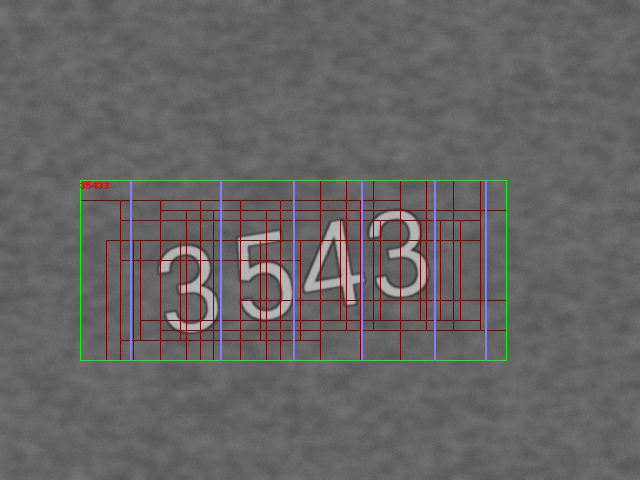
\includegraphics[width=0.35\linewidth]{fig/bad_examples_pipeline/cc904d6d-5202-422b-9a31-e8e49ddad840}
    }
    \caption{
      Examples of incorrectly transcribed digit strings. Repetition of digits (left).
      Missing digits (center). Low contrast images and small test size may result in character failing detection,
      resulting in a bounding box that is too small for segmentation and classification (right).
    }
    \label{fig:bad_examples_pipeline}
\end{figure}

As part of this project a proof-of-concept demo was implemented that detects and transcribes
strings of digits using a webcam. Example screenshots of this demo in action are shown in \figref{webcam}. As can be seen,
the system works in principle and successfully detects and transcribes digit sequences at
different angles of rotation (\figref{webcam}, (left) and (center)).
Regrettably, performance is lacking: even when running the OCR pipeline on a GPU (GTX 1060), the system struggles to deliver an acceptable frame rate.
It also struggles when the image is cluttered, as shown in \figref{webcam} (right), where
an additional edge is introduced. The false positives of the character detector at this edge
prevent the system from finding a text bounding box that is tight enough to enable successful transcription
of the digit sequence.

\begin{figure}[ht]
    \centering
    \makebox[\textwidth][c]
    {
      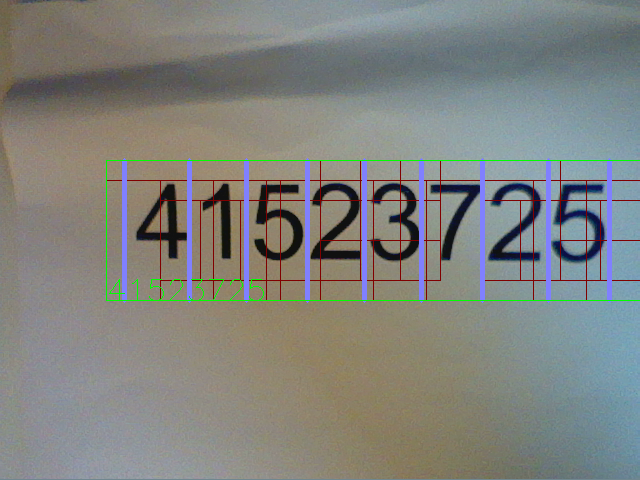
\includegraphics[width=0.5\linewidth]{fig/screenshots/eee8d50a-684a-4f54-8e89-3c4e729530c1}
      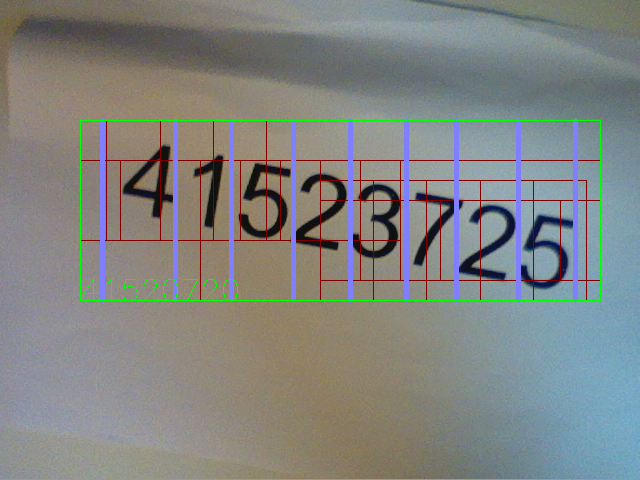
\includegraphics[width=0.5\linewidth]{fig/screenshots/861d0c35-3c77-4c95-8546-88976d6f2818}
    }
    \makebox[\textwidth][c]
    {
      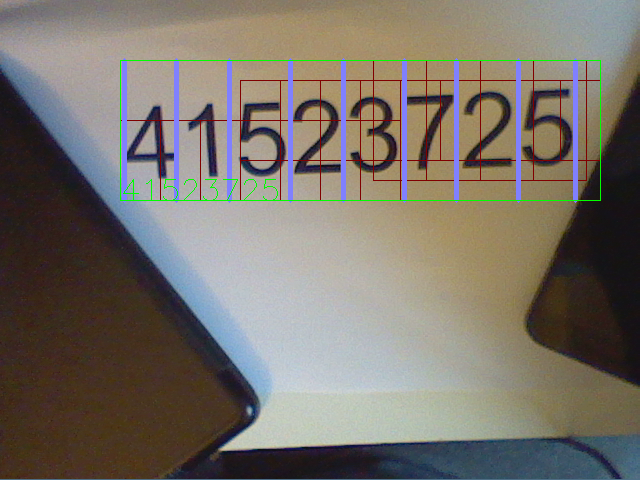
\includegraphics[width=0.5\linewidth]{fig/screenshots/0c64bcfc-61a5-4145-931e-1e68c99201c5}
      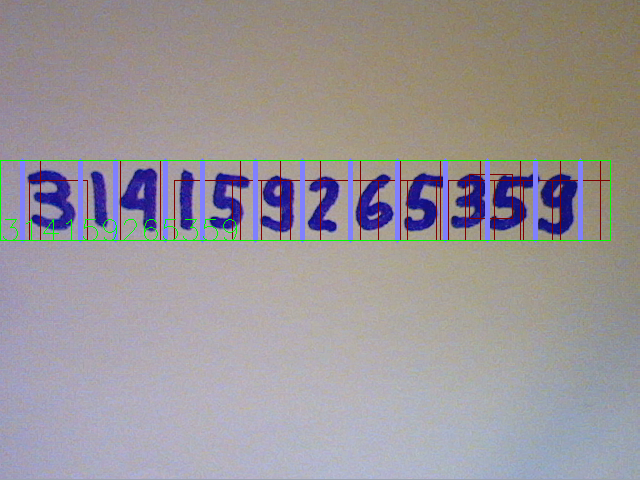
\includegraphics[width=0.5\linewidth]{fig/screenshots/33b6758a-5d0a-4725-8cef-74935f3d9174}
    }
    \caption
    {
      Screenshots of the proof-of-concept implementation of a text detection system using
      a webcam. Successful text detection (top left, top right) for different angles of rotation.
      Successful text detection in an image cluttered by high contrast edges (bottom left).
      Successful text detection of a handwritten number string (botton right).
    }
    \label{fig:webcam}
\end{figure}

\section{Conclusion}
Implementing a photo OCR pipeline is a challenging problem. Not only do all of the different stages
of the pipeline have to achieve a high level of accuracy, their performance also have a direct
impact on the later stages. If, for example the text detection stage does not extract a tightly
fitting bounding box, the segmentation and classification stages will receive character images
that are scaled down vertically, thus reducing their ability to perform at their maximum
accuracy.

Accuracy can be improved by increasing the spacial resolution and the number of intermediate scaling steps
of the sliding window text detection.
Both measures in turn will drastically increases the processing time per image. This problem is
further exacerbated if the system should also be able to extract text of small size because in this requires
upscaling of the source image prior to text detection.

Apart from the unfavorable accuracy/time trade-off, the sliding window algorithm suffers from an additional
drawback: The text detection classifier has to make accurate decisions based only on the contents
of a small section of the whole image. All surrounding contextual information is discarded, which
makes it very hard to reach a high accuracy. Does an edge detected in a window belong to a character
or is it the edge of a piece of paper? Is there an arc of a digit or does the background have
some coarse structure to it? These dilemmas either lead to many false positives if the
decision threshold is lowered or to incomplete text bounding boxes if the threshold is increased
too much which both decrease accuracy in certain applications. Consequently it is very hard
to implement a robust system that generalizes well over a broad range of applications and
would instead lead to specifically tuned versions for different purposes
(e.g. document scanning vs. extracting text from street view images).

Improving the sliding window algorithm could be achieved by a dividing text detection into
multiple phases. In \cite{Li2016}, candidate bounding boxes are first computed using a
simple CNN classifier which are then further filtered on multiple resolutions
based on heuristics from the problem domain (car license plate detection). In \cite{Jaderberg2016},
proposals are filter using a random forrest classifier and then further enhanced using a regression
technique.

Overall it seems that the sliding window algorithm, while relatively straightforward to implement
(if hard to optimize) and widely used, would better be replaced by a solution that can be trained
end-to-end and that takes more image context into account. One technique are R-CNNs \cite{Girshick2013,Jaderberg2016},
which use a selective search in image space to generate proposal regions that are then fed
into a CNN for classification. Another technique is YOLO (You Only Look Once, \cite{Redmon}) that
uses a grid of classifiers in order to directly predict the position and size of bounding boxes.
Finally, if the (maximum) length of the text is known for the application \cite{Goodfellow2013,Li2016}, this will also greatly simplify
the detection algorithm as, for example, the aspect ratio of the text bounding boxes can be used
to filter out false positives.

\newpage
\bibliography{main,web}
\bibliographystyle{ieeetr}

\end{document}
